


\chapter{Developing a Suitable MAS Framework: ASC2}
Agent-based modelling is a valuable tool in designing complex socio-technical systems. The chapter introduces an Agent-Oriented Programming (AOP) framework based on the Belief-Desire-Intention (BDI) model of agency. There are multiple BDI frameworks already introduced in the literature. Prior to development of ASC2, we tried to adapt and utilize multiple of these frameworks, while there were different advantages and disadvantages to each of them, in the end, the main reason that resulted in designing and developing yet another framework was firstly interoperability and and secondly maintainability. None of these framework allowed for seamless interoperability between agents and other mainstream software. Also, these frameworks had most of the agent's reasoning hard-coded into them which is detrimental to experimentation on alternate theories of an agents behavior. By getting inspirations from the design of previous works, the novelty of this framework is in relying on the Actor model, instantiating each intentional agent as an autonomous micro-system run by actors. The hypothesis behind this choice is that defining the agents via actors results in a more fine-grained modular architecture that is more modifiable and that the execution of agent-oriented programs is enhanced (in scalability as well as in performance) by relying on robust implementations of Actor models such as \textit{Akka}.


\section{Introduction}
Agent-based models have an intuitive mapping to behavioural descriptions, and for this reason are extensively used for modeling and simulations of social systems. However, \textit{agent-based programming} is not only relevant for simulation. Complex Cyber-Infrastructures like those used for data-sharing as digital marketplaces exhibit the double status of computational and social systems; regulating these infrastructures requires reproducing to a certain extent constructs similar to those observed in human reasoning (e.g. For which purpose is the agent asking access to the resource? On which basis is the infrastructure granting access?). For \textit{traceability} and \textit{explainability} reasons, decisions concerning actions need to be processed by the infrastructure as much as relevant operational aspects. Agent-based programming, by looking at computational agents as intentional agents, provides this level of abstraction available \textit{by design}. However, this raises concerns on how we can efficiently map logic-oriented agent-based programs into an operational setting, a problem motivating the present research.


% ASC2 is a higher-level logic-based DSL for specifying scripts for intentional agents, i.e. sets of behavioural responses to environment conditions that are expected to achieve certain purposes. The standard approach to these type of languages is to use them by means of an interpreter. This work reports on a experiment to approach the via a trans-compilation tool, i.e. translating such higher-level DSL to a lower-level executable language (in this case Scala) that can be then compiled and executed.


This chapter introduces ASC2, a logic-based AOP framework in which agents are modular micro-systems run by actors. To evaluate the feasibility of this approach for future developments, a first implementation of ASC2 based on Akka runnig on JVM is compared with three other relevant AOP frameworks (Jason \cite{Bordini2005}, ASTRA \cite{Astra} and Sarl \cite{Astra}) by means of 3 benchmarks (token ring, chameneos redux and service point), known to capture relevant patterns in concurrent applications. This performance evaluation shows that despite its relative youth and the new implementation approach, ASC2 is competitive against existing frameworks, making it worthy of further investigation.
% The initial performance evaluation shows that despite its relative youth and new implementation approach, ASC2 is competitive against existing frameworks, making it worthy of further investigation.

The chapter proceeds as follows: Section~\ref{sec:agere:background} provides some background on relevant concepts and related works. Section~\ref{sec:agere:method} presents the ASC2 framework. Section~\ref{sec:agere:evaluation} reports on the empirical experiments comparing ASC2 with other frameworks. Section~\ref{sec:agere:discuss} compares the frameworks qualitatively. A note of future developments ends the chapter.


\section{Background}
\label{sec:agere:background}
\subsection{Agent Oriented Programming}

Agent-Oriented Programming (AOP) is a programming paradigm that uses mental attitudes to model autonomous computational agents. Introduced in 1993 by Shoham \cite{shoham1993agent}, it has attracted increasing attention ever since and is believed to provide an effective abstraction to approach complex software systems (e.g. \cite{Sarl}). In the beginning it was presented as a specific version of Object Oriented Programming (OOP): whereas object classes contain arbitrary components, agent types share the same types of mental states and of structural relationships/mechanisms involving those states. 


\subsection{Belief-Desire-Intention (BDI) Model}
Having its roots in a theory of mind \cite{bratman1987intention}, and so referring to categories that are used typically to address human behaviour to describe agents, the \textit{belief-desire-intention} (BDI) model \cite{Rao1995} has been extensively investigated as basis to represent computational agents that exhibit rational behaviour \cite{Herzig2017}. 
% uses taxonomies that are used typically to address human behaviour to describe agents.
\textit{Beliefs} are the factual (and possibly inferential) information the agent has about itself or its environment. \textit{Desires}, in their simplest form, are objectives the agent wants to accomplish. % \Gio{(i.e. facts desired to be true)}.
%in the environment. 
\textit{Intentions} are the courses of action the agent has committed to. In practice, BDI agents include concepts of \textit{Goals} and \textit{Plan}. Goals are instantiated desires % associated to reactive behaviors to certain events 
and plans are abstract specifications relating a goal to the means of achieving that goal (intentions become commitment towards plans). Multiple programming languages and frameworks have been introduced based on the BDI model, as AgentSpeak(L)/Jason \cite{RaoAS1996,Bordini2005}, 3APL/2APL \cite{Dastani2APL}, GOAL \cite{Hindriks2009a} and IMPACT \cite{IMPACT}.


\subsection{Actor Model}
The Actor model, introduced in \cite{Hewitt}, is a mathematical theory that treats \textit{actors} as the primitives of computation \cite{hewitt2010actor}. Actors are essentially reactive concurrent entities. % that use message passing as the basis of their communication. 
When an actor receives a message it can %concurrently 
send messages to other actors; \textit{spawn} new actors; modify its reactive behavior for the next message it receives.
Originally proposed as a tool for the theoretical understanding of concurrency, the Actor model serves now as the basis of several production-level solutions for distributed and asynchronous systems, and for reactive programming. These solutions include: Akka \cite{AKKA}, a library developed for the JVM environment, enriched by a strong community with multiple complementary tools for distributed environments and stream processing; the C++ Actor Framework (CAF) \cite{CAF}, a library %written in C++ 
for creating concurrent programs in C++; Pony \cite{PONY1,PONY2}, an actor language for building robust parallel systems by providing data-race free isolation for actors. A comprehensive overview and benchmark over these works can be found in \cite{RunActor}. 


\subsection{Related Work}
Multiple AOP and BDI frameworks have been introduced proposing diverse approaches towards language, execution model, reasoning process, etc. Jason \cite{Bordini2005} is plausibly the most known (e.g. it is the most used choice in the Multi-Agent Programming Contest \cite{mapc}), and has been constantly developed in the last 15 years. It is implemented in Java and is essentially an \textit{interpreter} for a logic-based DSL, namely an extended version of AgentSpeak(L) \cite{RaoAS1996}.  Two recent frameworks inspired by Jason are Pyson \cite{pyson} and LightJason \cite{LJ}. Pyson is an interpreter implemented in Python and uses \verb+MapReduce+ technology as execution infrastructure in order to achieve better scalability specifically w.r.t. the number of agents. LightJason is a BDI framework based upon a variation of AgentSpeak(L) and whose interpreter aims to improve the scalability of Jason by implementing a concurrent platform following best practices in software engineering.

ASTRA \cite{Astra} is yet another framework inspired by AgentSpeak(L)/Jason and is also implemented in Java, but, unlike Jason, it is not an interpreter. ASTRA relies on a \textit{compilation} approach: through a build pipeline the DSL is first translated to pure Java code and then the Java code is compiled to byte-code for execution. In contrast, the Sarl \cite{Sarl} framework has not been introduced as a BDI platform and then it does not use the same abstractions. Nonetheless it is an AOP framework written in Java that also uses compilation, and for these reasons it is relevant for the current study.

% and that puts scalability amongst the requirements it aims to satisfy. 

Although several AOP/BDI frameworks have been introduced in the recent years (all hinting to problems of scalability), there is a small amount of empirical data available about how they perform in comparison to each other. The most notable exception is  \cite{Cardoso2013}, in which multiple actor and agent frameworks (2APL \cite{Dastani2APL}, GOAL \cite{Hindriks2009a}, Jason and Akka) are benchmarked. Their results showed that Jason outperformed other BDI frameworks by far and scaled almost on par with Akka. However, at that time (2013), none of these newer frameworks had been introduced yet, and Akka had not the support it has today. Strangely enough, none of these new AOP frameworks has the Actor model at their foundation. The present chapter aims to investigates part of this gap.


\section{AgentScript Cross-Compiler (ASC2)}
% In this section the ASC2 framework is introduced. 
% At its core 
This section introduces ASC2, however, as this framework is central to this thesis, detailed descriptions of different parts related to specific concepts is presented in the respective sections. The ASC2 framework consists of: (a) a logic-based Agent-Oriented Programming DSL; (b) an abstract agent run-time architecture; (c) a translation method that generates executable models from models specified by the DSL; (d) tools that support the execution of models. We provide here a brief overview on these components.

\subsection{ASC2 DSL}
\label{section_dsl}

The ASC2 DSL has a very close syntax to AgentSpeak(L) language and includes some of the extensions provided by Jason. The main components of the DSL are (1) initial beliefs, (2) initial goals, and (3) plan rules. Initial beliefs are a set of Prolog-like facts and inferential rules that are potentially non-grounded declarative rules (Prolog-like), used to infer beliefs from beliefs. Initial goals designate the first intentions to which the agent commits. These can be used as a way to initialize an agent in their environment, and maybe start interacting with other agents. 

Plan rules are potentially non-grounded reactive rules in the form $e : C \Rightarrow H$ that map different internal or external events $e$ (e.g, \textit{goal adoption}, \textit{belief-update}) to a sequence of executable steps $H$ called the \textit{plan body} which the agent will perform in response to the event. The steps of a plan body can include belief query, belief update, sub-goal adoption, primitive actions, variable assignment, and control flow structures (loops and conditionals). Each plan also has a context condition $C$ which is a Prolog-like expression that represents when that plan is applicable. The full grammar definition of ASC2's DSL is presented in Listing~\ref{listings:asc2grammar}.

\begin{listing} 
\begin{minted}[escapeinside=00,mathescape=true]{js}
agent           0$\rightarrow$0 beliefs initial_goals plans
beliefs         0$\rightarrow$0 (term '.')*
initial_goals   0$\rightarrow$0 ('!' atomic_formula '.')*
plans           0$\rightarrow$0 (plan '.')*
plan            0$\rightarrow$0 ( '@' atomic_formula )*
                trigger_event ( ':' context )
                '=>' body_definition '.'
trigger_event   0$\rightarrow$0 ( '+'|'-'|'+!'|'-!'|'+?' ) atomic_formula
context         0$\rightarrow$0 term
body_definition 0$\rightarrow$0 body_formula ( ';' body_formula )*
body_formula    0$\rightarrow$0 ( '!'|'+'|'-' ) literal
                |  loop
                |  conditional
                |  primitive_call
                |  <VARIABLE> '=' term
term            0$\rightarrow$0 <VARIABLE>
                |  '(' term ')'
                |  <INTEGER> | <FLOAT> | <STRING> | 'true' | 'false' 
                |  <ATOM> '(' term_list ')'
                |  term operator term
                |  'not' term
                |  '[' term_list ( '|' term )? ']'
                |  <ATOM>
                |  primitive_call
atomic_formula  0$\rightarrow$0 <ATOM>
                |  <ATOM> '(' term_list ')'
literal         0$\rightarrow$0 <VARIABLE> 
                |  atomic_formula               
term_list       0$\rightarrow$0 term ( ',' term )*
operator        0$\rightarrow$0 '**'|'*'|'/'|'mod'|'+'|'-'|'='
                |'=='|'!=='|'!='|'<'|'<='|'>'|'>='|'is'|'>>'
                |'^'|'&&'|'||'|':-'
primitive_call  0$\rightarrow$0 '#' <ATOM> ( '.' <ATOM> )* '(' term_list? ')'
loop            0$\rightarrow$0 'for' '(' <VARIABLE> 'in' term ')' 
                '{' body_definition '}'
conditional     0$\rightarrow$0 'if' '(' term ')' '{' body_definition '}'
                ('else' 'if' '(' term ')' '{' body_definition '}')*
                ('else' '{' body_definition '}')?
\end{minted}
\caption{AgentScript's DSL grammar defenition}
\label{listings:asc2grammar}
\end{listing}%\label{listings:asc2grammar}


An example of an ASC2 DSL that shows part of the script for a domestic robot is presented in Listing~\ref{lst:domestic_robot}, where lines 2-4 are initial beliefs, line 6 is an inferential rule, line 9 is an initial goal and lines 12-15 define an example plan. This script is further expanded on in the next chapter.

\begin{listing}[!h]
\begin{minted}[fontsize=\small,linenos]{prolog}
% initial beliefs and inferential rules
main(fish). soup(veg). wine(white).
restaurant(french).
at(home).

meal(S,M,W) :- soup(S), main(M), wine(W).

% initial goals
!go_order(french,meal(veg,meat,white)).

% plans
% P1
+!go_order(Loc,Meal) :
        restaurant(Loc) && not at(Loc) =>
        #move_to(Loc);
        !order(Meal).
...
\end{minted}
\caption{An example script of ASC2 DSL}
\label{lst:domestic_robot}
\end{listing}

%  An example of initial goals for the domestic robot agent can be:
% \begin{minted}[fontsize=\small]{prolog}

% \end{minted}

%  An example of a plan in the domestic robot agent that tells it to go a location and order a meal:
% \begin{minted}[fontsize=\small]{prolog}
% +!go_order(Loc,Meal) :
%     restaurant(Loc) && not at(Loc) =>
%         #move_to(Loc);
%         !order(Meal).
% \end{minted}

% Note that this plan is applicable only if the location is believed by the agent to be a restaurant, and, the agent believes it is currently not at that location. The plan body has two steps, one is a primitive action \asc{#move_to(Loc)} which is a low level call to a function and the second one is adoption of a sub-goal \asc{!order(Meal)}.

%When a plan body $f$ is matched with an event $e$, it is said that $f$ is \textit{relevant} for $e$. Each plan also has a context condition $c$ which is a Prolog-like expression. When a plan $f$ is relevant for $e$ and also $c$ holds, it is said that the $f$ is \textit{applicable} for $c$.  The grammar definition of ASC2's DSL is presented in Listing~\ref{listings:asc2grammar}. % \textcolor{red}{how much more does this section need to expand?}




\subsection{ASC2 Run-time Architecture}
\label{section_arch}
ASC2 is primarily motivated by AgentSpeak(L)/Jason as a starting point, and in its default setting it is designed to have the (almost) the same functional architecture. However, from a structural perspective, ASC2 is novel in the sense that it utilizes actor model to instantiate agents as actor micro-system. Because of this, the run-time architecture of ASC2 agents can and should be inspected from both functional and structural perspectives. 

\subsubsection*{ASC2 Functional Architecture}
From a functional perspective, ASC2 agents (by default) conceptually follow a reasoning flow very close to the reasoning cycle defined by AgentSpeak(L)/Jason. An ASC2 agent consists of a set of beliefs $B$ called belief base, a set of plans $P$ called plan library, a set of events $E$, a set of intentions $I$, and three selection functions: $S_E$,$S_O$,$S_I$. When the agent receives an (internal or external) event or adopts a goal, it is added to $E$. The selection function $S_E$ selects an event to process from $E$.
%. 

% \begin{definition}
% [Plan] A (reactive) plan is specified by $e : C \Rightarrow H$ where $e$ is a triggering event, $C$ is a formula capturing context conditions, and $H$ is a sequence of sub-goals or actions to be performed at the occurrence of the trigger event.
% \end{definition}

Then, this event is matched with the triggering events in the heads of the plans in $P$. The plans that their triggering event unifies with this event are called \textit{relevant plans} and their unifier is called the \textit{relevant unifier}. Then for each relevant plan, the relevant unifier is applied to the context condition of that plan, and by querying against $B$ a substitution is created such that the context is a logical consequence of $B$. The composition of relevant unifier with this substitution is called an \textit{applicable unifier}. 

% \begin{definition}
% [Relevant plan] A plan in the form of $e : C \Rightarrow H$ is a \textit{relevant plan} with respect to an event $\epsilon$ iff there exists a most general unifier $\sigma$ such that $\epsilon\sigma = e\sigma$. Then, $\sigma$ is referred to as the relevant unifier for $\epsilon$.
% \end{definition}

% \begin{definition}
% [Applicable plan] A plan in the form of $e : C \Rightarrow H$ is an \textit{applicable plan} with respect to an event $\epsilon$ iff there exists a relevant unifier $\sigma$ for $\epsilon$ and there exists a substitution $\delta$ such that $C\sigma\delta$
% is a logical consequence of belief base $B$. The composition $\sigma\delta$ is referred to as the applicable unifier for $\epsilon$ and $\delta$ is referred to as a \textit{correct answer substitution}.
% \end{definition}


As for each event there could be multiple applicable unifiers, the selection function $S_O$ chooses one of these plans or options and applying the applicable unifier to that plan creates an instantiated plan, i.e, an intended means for the event which will be added to a new or existing intention. Then the $S_I$ function selects an intention which will be executed. Figure~\ref{fig:asc2func} presents an overview of the functional architecture embedded in ASC2 agents.

\begin{figure}[t!]
  \centering
  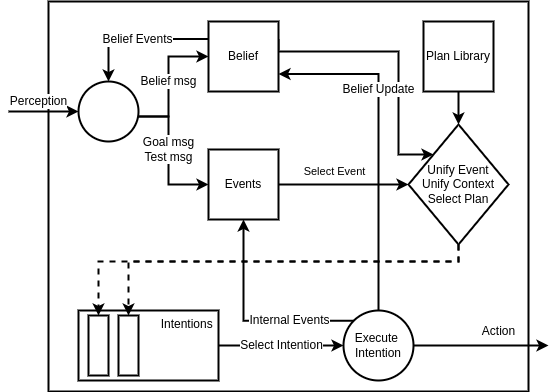
\includegraphics[width=0.70\linewidth]{ch2/asc2arch.drawio.png}
  \caption{ASC2's functional architecture}
  \label{fig:asc2func}
\end{figure}


Taking the example script in Listing~\ref{lst:domestic_robot}, Suppose the agent receives and event in the form of: 
\begin{minted}[fontsize=\small]{prolog}
!go_order(french,meal(veg,meat,white))
\end{minted}
\noindent For this event, plan P1 is relevant with unifier:
\begin{minted}[fontsize=\small]{prolog}
{Loc/french, Meal/meal(veg,meat,white)}
\end{minted}
Then applying this unifier to the context condition of that plan will result in the expression:
\begin{minted}[fontsize=\small]{prolog}
restaurant(french) & not at(french)
\end{minted}
Which indeed is a logical consequence of the agents beliefs, meaning this plan is applicable with the same unifier as before (i.e., the query does not add any new substitutions). Then, by applying this substitution to the plan itself will result in:
\begin{minted}[fontsize=\small]{prolog}
+!go_order(french,meal(veg,meat,white)) :
    restaurant(french) & not at(french) =>
    #move_to(french);
    !order(meal(veg,meat,white)).
\end{minted}

The steps in the body of the instantiated plan become an intended means for the agent to execute. The first step \asc{#move_to(french)} is simply a function call. In ASC2, this could be any callable entity on the JVM's execution classpath. In this example we are assuming that this call somehow relocates agent to the location specified as the parameter. The second step is \asc{!order(meal(veg,meat,white))} which is a sub-goal. In functional terms a sub-goal is processed by the agent as an internal event that will follow the same plan selection process.

This process is better described in ASC2 as a reasoning flow instead of a reasoning cycle. This is because unlike what is typically the case in BDI frameworks, ASC2 does not implement an explicit synchronous reasoning cycle. As a result the two selection functions $S_E$ and $S_I$ are asynchronous: when an event arrives, it will be processed in an asynchronous manner given there are free resources available to the agent. Or, when a new intent is created, it will be executed asynchronously given there are free resources available. In effect, the sets $E$ and $I$ are priority queues and $S_E$ and $S_I$ are sorting functions that define the priority of the entities in these queues. The default implementation for both is a simple first-in-first-out (FIFO) algorithm. A new event or an intention will be selected by their respective selection function when processing resources, namely threads from a thread pool become available.



% As this work focuses on the goal refinement, the following formal definitions namely plans, relevant plans, and applicable plans are reiterated from \cite{RaoAS1996}. 





% \Gio{[here we should write a bit about variables, constants, unification and unifiers.]}
% \Mos{Giovanni can write this}


%\noindent For the given definitions, only relevant plans may be applicable. 

% \paragraph{Domestic Robot Agent}
% To demonstrate the full functional plan instantiation process of our agent, imagine a domestic robot that upon request can go to a restaurant and order a three course meal. The script for such agent is presented in Listing \ref{lst:domestic_robot_1}. 
% %\footnote{In the excerpts we modified slightly the AgentSpeak(L) syntax, replacing ``\texttt{<-}'' with ``\texttt{=>}'', to further distinguish the reactive, forward nature of these rules w.r.t. the backward chaining derivation of Prolog rules ``\texttt{:-}''.} 
% The agent has two plans for going to a restaurant and ordering a meal, the first plan (P1) is \textit{applicable} if the agent is not at a restaurant at the moment, which means a step of moving (\asc{#move_to} primitive action) is needed prior to ordering the meal, the second plan (P2) is applicable if the agent is already at the restaurant which means the agent will just adopt the goal of ordering the meal. There is also one plan for ordering the meal (P3) which is applicable if the agent has the belief that the meal it wants to order exists.

% \begin{listing}[t]
% \centering
% \begin{minted}[fontsize=\small]{prolog}
% % initial beliefs
% main(fish). main(meat). soup(veg). soup(fish).
% wine(white). wine(red).
% restaurant(french). restaurant(italian).
% at(home).
% % inferential rules
% meal(S,M,W) :- soup(S), main(M), wine(W).

% % plans
% % P1
% +!go_order(Loc,Meal) :
%         restaurant(Loc) && not at(Loc) =>
%         #move_to(Loc);
%         !order(Meal).
% % P2
% +!go_order(Loc,Meal) :
%         restaurant(Loc) && at(Loc) => 
%         !order(Meal). 
% % P3
% +!order(meal(S,M,W)) : 
%         meal(S,M,W) => 
%         #ask_waiter(meal(S,M,W)).
% \end{minted}
%     \caption{Domestic robot agent's script}
%     \label{lst:domestic_robot_1}
% \end{listing}%
% \noindent Suppose the agent receives and event in the form of: 
% \begin{minted}[fontsize=\small]{prolog}
% !go_order(french,meal(veg,meat,white))
% \end{minted}
% It will put it in the event queue, assuming this is the only event the agent selects it for processing. For this event, both plans (P1) and (P2) are relevant with unifier $\sigma$:
% \begin{minted}[fontsize=\small]{prolog}
% {Loc/french, Meal/meal(veg,meat,white)}
% \end{minted}
% Assuming that the belief base of the agent contains the beliefs \asc{restaurant(french)} (meaning that there exists a French restaurant) and \asc{at(home)} (meaning that the agent is at home), then only the first plan will be an applicable plan for this event, and the applicable unifier will be the same as the relevant unifier. This entails that only plan (P1) will be instantiated as: 
% \begin{minted}[fontsize=\small]{prolog}
% +!go_order(french,meal(veg,meat,white)) :
%     restaurant(french) & not at(french) =>
%     #move_to(french);
%     !order(meal(veg,meat,white)).
% \end{minted}

% As a next step, this instantiation becomes an intention of the agent, and assuming it is the only intention, the agent selects it for execution, the first step \asc{#move_to(french)} is simply a function call. In ASC2, this call could be any callable entity on the JVM's execution classpath. In this example we are assuming that this call somehow relocates agent to the location specified as the parameter. The second step is \asc{!order(meal(veg,meat,white))} which is a sub-goal. In functional terms a sub-goal is processed by the agent as an internal event that will have the same plan and intention selection process.


% Note that in case the agent at any step had more than one event to select from, more than one plan or applicable unifier, or more than one intention, then the selection function would have been called to select one of the options.


\subsubsection*{ASC2 Structural Architecture}
The structural architecture of ASC2 agents is based on the Actor model. Each agent consists of multiple actors with different roles: (\romannumeral 1) an \textbf{Interface} actor, (\romannumeral 2) a \textbf{Belief Base} actor, (\romannumeral 3), an \textbf{Intention} \textbf{Pool} actor and (\romannumeral 4) $N \ge 1$ \textbf{Intention} actors. Each agent has also non-actor components: (1) a plan library, and (2) one or more belief bases. An overview of this architecture is presented in Figure~\ref{fig:asc2arch}.
%\begin{itemize}
%    \item An Interface actor
%    \item A Belief Base actor
%    \item An Intention pool actor
%    \item $N \ge 1$ Intention actors
%\end{itemize}

The plan library of the agent consists of a set of plan rule objects in the form \verb+{e,c,h}+, where \verb+e+ is an object that can be matched and unified with event messages to determine if a plan rule is relevant for that event, \verb+c+ is an expression object that can be sent to the Belief Base actor to determine if the plan is applicable and \verb+h+ is a function representing the body of the plan.

The belief base(s) of the agent can be in practice any type of storage technology. To interface an arbitrary belief base into the agent architecture a translation function needs to be implemented for mapping the query messages into the queries of that belief base and vice versa, translating the responses into result messages.\footnote{For the benchmarks presented in this work we used a lightweight open-source Prolog reasoning engine implemented in Scala called \textit{Styla}, available at \url{https://github.com/fedesilva/styla}. %, % \cite{Styla}
The library was minimally modified and is available at \url{https://github.com/mostafamohajeri/styla}.}

\begin{figure}[t!]
  \centering
  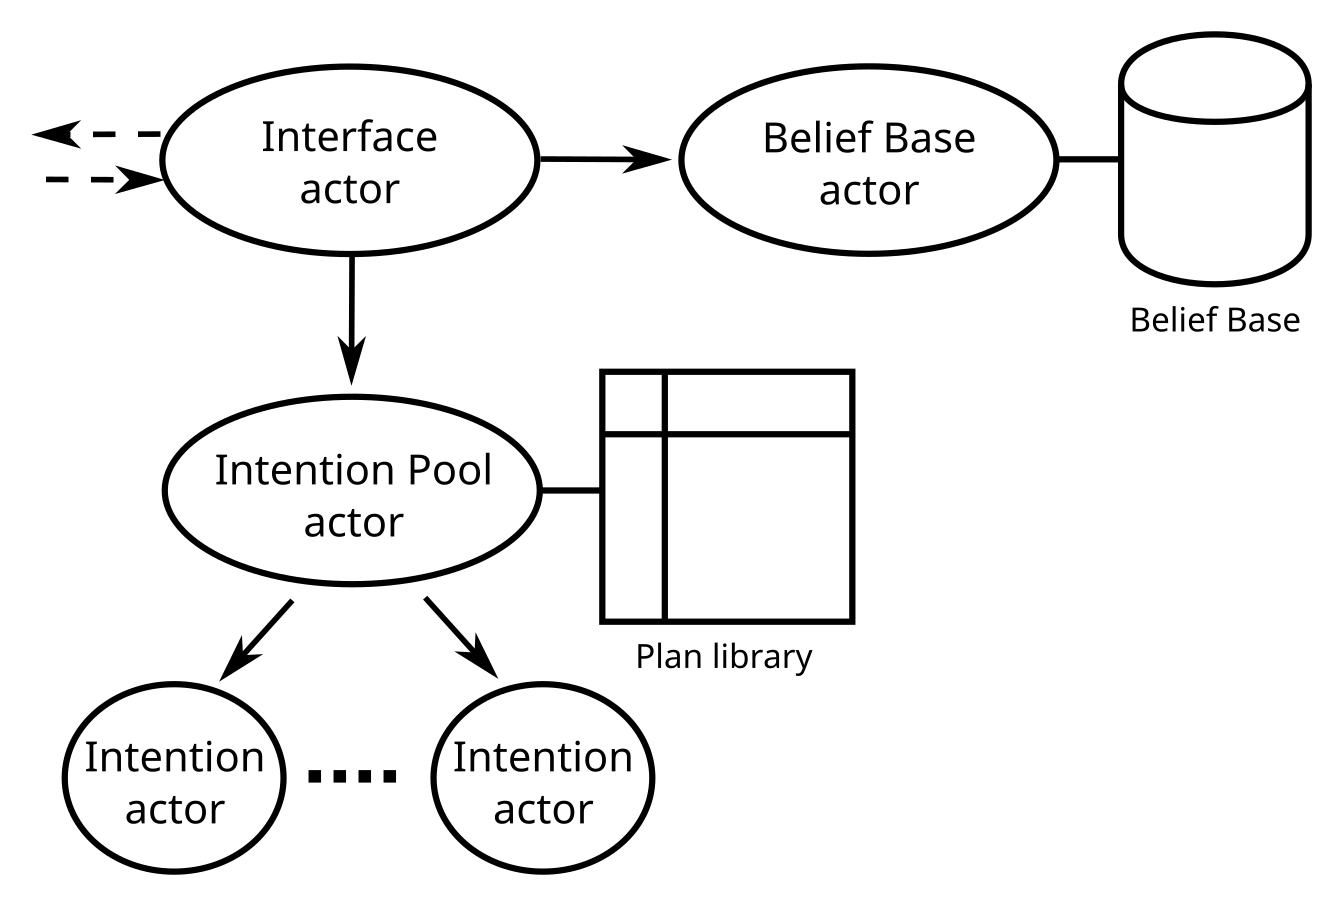
\includegraphics[width=0.70\linewidth]{ch2/arch3.png}
  \caption{ASC2's structural architecture}
  \label{fig:asc2arch}
\end{figure}

\subsubsection{Interface Actor}
The Interface actor acts as the main entity of the agent. It initializes the Belief Base and Intention Pool actors and then sends the initial beliefs and inferential rules to Belief Base actor as \textit{assert} messages and initial goals to Intention pool actor as \textit{achieve} messages. This actor is the only component of the agent that is accessible from the environment and the other agents: all incoming messages and events must go though this actor and any message sent from this agent will indicate the Interface actor as the sender of message. When the Interface actor receives a new message $m$, based on the type of the message it will either process it itself if $m$ is a control messages, (e.g, \textit{halt}), forward it to Belief Base actor if $m$ is an assert message (e.g, \textit{perception}) or forward it to Intention Pool actor if $m$ is an achieve message (e.g, \textit{request}).


\paragraph{Communication Interface}
All the external communications of the agent are transmitted through a communication layer. This layer is one of the dependencies that is injected into the agents at initialization time. This allows the designer to implement this layer with any technology (e.g., REST API, gRPC, Message Queues) and inject it into agents to allow them to communicate with other agents (and other entities) using that technology without the need to modify the framework or even the script of the agents.

The communications interface of the agents is based on speech act preformatives. On a practical level, they are implemented with actions like \mintinline{text}{#achieve} which relays an achievement goal event, \mintinline{text}{#tell} and \mintinline{text}{#untell} which relay belief-update events, and \mintinline{text}{#ask}/\mintinline{text}{#respond} which can be used between agents as synchronous communication with test goal events.


\subsubsection{Belief Base Actor}
The Belief Base actor maintains the connection between other components of the agent and any data storage/reasoning engine that is used as the belief base. This actor accepts query messages (\textit{retract}, 
\textit{assert} and \textit{unify}) and responds with result of the query. The technology of the data storage(s) is abstracted behind this actor and it can be changed by the programmer without affecting the rest of the framework. The specific implementation of the belief-base is injected to the agent initialization time. % Note that also inferential rules can be seen as \textit{integrity constraints} that the belief base is required to enforce. 
Apart from processing queries, the Belief Base actor also feeds back \textit{belief-update} events to the Interface actor. The semantics of when these events should be created are externalized to the core of architecture and can be programmable by the designer. This is the inversion of control as the belief base can control other components by sending messages to them.

\subsubsection{Intention Pool actor}
The Intention Pool actor receives events from the Interface actor and processes them. To process a received event \verb+v+, the set of relevant plan rules \verb+{e,c,h}+ are selected from the plan library by matching and unifying \verb+v+ against \verb+e+. Then these relevant plans are fetched from the plan library and sent to an idle Intention actor. The Intention pool actor can spawn $N$ Intention actors, where the configurable number $N$ dictates the number of concurrent intentions each agent can have at each instant. This actor uses a prioritized mailbox that sorts the messages based on the externalized programmable priority function $S_E$ and a new event is processed only if there are idle Intention actors to forward it to. This mechanism makes sure that as long as there are no resources available, new events stay in the mailbox to be re-prioritized by $S_E$ and when an idle Intention actor becomes available the event with the highest priority is processed \footnote{In the current implementation, the Intention pool actor exploits the \textit{Router} feature of Akka.}. % is used to implement the Intention pool actor.

\subsubsection{Intention Actor}
An Intention actor is a reusable unit of execution for the agent. It receives an event \verb+v+ alongside a set of plan rule objects \verb+{e,c,h}+ from the Intention Pool actor for execution. The execution consists of three phases: (\romannumeral 1) the applicability of each plan rule is checked by sending a query message containing \verb+c+ to the Belief Base actor; (\romannumeral 2) from the set of applicable plans, one is selected by the externalized programmable function $S_P$ for execution; (\romannumeral 3) the function  \verb+h+ of the selected plan is executed by the Intention actor. After the execution of \verb+v+ is completed either by success or failure status, a message is sent to the actor which originally requested \verb+v+ containing the completion status and also a message is sent to Intention Pool actor signaling that this actor is now idle.


\subsection{Translation Method}
The translation method is designed to compile the models specified with the ASC2 DSL described in \ref{section_dsl} into agents with the architecture described in \ref{section_arch}. 

For each entity of the DSL, a mapping is defined to generate the code in the executable underlying language that can instantiate the objects with the desired semantics at run-time. The translated entities are then fitted in the abstract architecture to form an executable agent program.

\subsubsection{Terms and Expressions}
The ASC2 DSL uses Prolog-style terms and expressions. In the translation of an script written in the DSL, each term and expression (including inferential rules) maps to a \verb+Term+ or \verb+Expression+ object which encapsulates the parsed data (potentially containing nested \verb+Term+s and \verb+Expression+s).

Any expression in ASC2 can be analysed in two ways: (1) external to the script by querying the belief-base, and, (2) locally as part of the low-level code. The first approach makes use of any data-storage engine utilized by the belief-base. This process is by default present in checking the context conditions of plans, but can also be used at any point in the agent's script; in our example the expression:
\begin{minted}[fontsize=\small]{prolog}
restaurant(french) & not at(french)
\end{minted}
\noindent can be checked against the belief base to check if it is true. This approach utilizes the full capacity of the belief-base but is also less efficient. The second type of expression are locally calculated, and for example are used in control flow structures \asc{if/else} or variable assignments. As an example, if in the context of execution of a plan we have a variable \asc{Loc} that is grounded by the string value \asc{"french"}, the statement:
\begin{minted}[fontsize=\small]{prolog}
Loc + "_restaurant" == "french_restaurant"
\end{minted}
\noindent can be calculated locally to boolean value \asc{true} without the need to query the belief-base. Intuitively this second approach does not utilize the capabilities of the belief-base but the local nature of its translation ---it is calculated locally by the underlying language--- can be very efficient.

\paragraph{Access to the Lower-Level Language} As consequence of an approach based on compilation, the DSL provides direct access to any object or function available in the agent's name space\footnote{In the Scala implementation, any object or function which is accessible via the Java class path.}. These lower-level access statements, indicated by the token \verb+#+, are translated literally to the same statement in the underlying language. This capability provides fast and seamless reuse of libraries already established for the underlying language.

 %alongside implicit and explicit type conversions,

\subsubsection{Initial Beliefs/Goals and Inferential Rules}
At syntactic level, initial beliefs and inferential rules are logic-style expressions, and as such they translate to an \verb+Expression+ object counterpart. Initial goals are a combination of a prefix (\verb+!+, designating the adoption of a new goal)
and a term and they translate to a \verb+Goal+ object encapsulating the prefix and a \verb+Term+ object.

\subsubsection{Plan Rules}
A plan rule $<e,c,h>$, should be translated into the object \verb+{e,c,h}+ which will be part of the plan library. The triggering event of the plan rule $e$ consists of a trigger (one of \verb#+!,-!,+?,+,-#) and a term $t$. The triggers convey the relevance of the plan to different event types while $t$ can be seen as the payload of that event; \verb#+!# relates to adoption of a new goal, \verb#-!# relates to failure of a goal, \verb#+?# relates to test goals, \verb#+# and \verb#-# respectively relate to assertion and retraction of a belief. The triggering event $e$ then translates to an \verb+Event+ object which encapsulates the trigger and the translated \verb+Term+ object of $t$. The context condition $c$ is an expression and translates to an \verb+Expression+ object which can be sent to the Belief-Base actor in a synchronous manner, and the response to that message determines if the plan is applicable in the current context and also returns the substitution for the variable (if any). The plan body $h$ of a plan rule consist of zero or more steps. %and each step can be one of the plan step types. 
%The plan body 
It is translated into a function \verb+h+, which contains the steps of $h$ as imperative lines of code implemented in it. Each type of step is translated differently as is described below.



\paragraph{Primitive Actions}
A primitive action of the form \verb+#h(...)+ %for an agent 
is translated into a lower-level call to a function \verb+h+ defined in the underlying language with its respective parameters. % Like other low-level access statements these can be any function available on the name space of the agent's object. 
% A step that is indicated by the parser as a primitive action, is translated into a function call 

\paragraph{Variable Assignments}
Variable assignments in form of \verb+V = exp+ are used to (re-)assign the result value of an expression \verb+exp+ to a variable \verb+V+. ASC2 uses an internal map-like approach to store variables that also manages variable scopes, meaning that each code block (e.g, plan body, condition block) holds a map of all variables declared in that scope which also inherits the variables in its parent scope. A variable assignment is translated to an append operation for the variable map by using the $V$ as the key and \verb+exp+ as the value.

\paragraph{Belief Updates}
Belief update steps are composed of a prefix \verb|+,-| and a term $t$. The prefixes respectively mean assertion and retraction. As the belief base of the agent is abstracted by the Belief Base actor, a belief update step is a blocking message to the Belief Base actor containing the prefix and the \verb+Term+ object of $t$.

\paragraph{Sub-Goal Adoption}
Task decomposition is crucial component of BDI-like agents and in essence is the ability to adopt sub-goals depending on the context of a plan. At the syntactic level, a (sub-)goal adoption is a prefix (e.g, \verb+!,?+) plus a term $t$. The prefixes respectively mean achievement and test goals. In the translation method a sub-goal adoption step is translated as two phases, (\romannumeral 1) a plan selection by using $S_P$ is done to select and fetch a plan rule object \verb+{e,c,h}+ from the plan library, (\romannumeral 2) the function \verb+h(...)+ is called with any parameters that $t$ may have as the arguments of \verb+h+.

\paragraph{Control Flow Structures}
The compilation method of ASC2 supports a  straightforward mapping of simple control flow structures such as loops and conditionals to their executable counterparts. The translation of these control structures to the underlying language is performed one-to-one; for example an \verb+if/else+ in the DSL is simply translated to an \verb+if/else+ in the underlying language.

\subsection{Tools for Execution}
The architecture of ASC2 agents is based on actors and for their execution these actors require an \textit{actor system} that \textit{spawn} and \textit{start} them. Additionally, a message \textit{transportation layer} needs to be specified to enable communication between agents. The framework remains agnostic with respect the transportation layer as long as there is an interface to convert messages from and to ASC2's message protocol.

Our current implementation of ASC2 is written in Scala and is based on the Akka framework. In addition to a compiler\footnote{Source code: 
\url{https://github.com/mostafamohajeri/scriptcc-translator}.}, it includes a minimal infrastructure that is able to spawn and start the compiled agents% \cite{CCTranslator}
\footnote{Source code: \url{https://github.com/mostafamohajeri/agentscript}.
%of the execution framework can be found in \cite{AgentScript}
}. The transportation layer makes simply use of Akka's typed messages, but other solutions can be easily integrated.



\section{Benchmarks}
\label{sec_bench}

The following section proposes quantitative comparisons between the ASC2 framework and three other frameworks: Jason (\verb+v2.5+), ASTRA (\verb+v1.0.0+) and Sarl (\verb+v0.11.0+). Jason \cite{Bordini2005} was chosen because, like ASC2, it uses a language based on AgentSpeak(L), is implemented in Java and as reported by \cite{Cardoso2013} potentially outperforms other BDI frameworks. ASTRA and Sarl are both also implemented in Java, but, more importantly, like ASC2, rely on a compilation approach. %which makes them a good candidate for comparison.

Performance comparison is effectuated by means of two fairly standard benchmarks (token ring, chameneos redux), close to what has been presented in \cite{Cardoso2013}. The main difference w.r.t. \cite{Cardoso2013} is the metrics, as we separate the interpretation/setup time from the execution time, to present better insights on how these frameworks operate. %while in \cite{Cardoso2013} they are considered together. 
An additional benchmark (service point) was also performed to assess the ability of the frameworks to allow concurrent decomposition of tasks inside the agents. The benchmarks were performed on a {Debian GNU/Linux 10} machine with an 8 core {Intel(R) Xeon(R) CPU E5-1620 v4 @ 3.50GHz} CPU and {64GB} of RAM using Java version {11} with {GraalVM 20} JRE.  Each benchmark was performed $10$ times and the JVM was stopped between each run to avoid the impact of one experiment on the next. %The results are further discussed in section \ref{sec:discussion}.

In the first two benchmark scenarios, three metrics are recorded: (1) total interpretation/setup time, including agent creation time, (2) internal execution time measured from the instant that the first agent starts until the completion of the test, and (3) CPU core load. Execution and data gathering is controlled by a Python script that runs the benchmarks in the desired dimensions and records the metrics\footnote{Source code: \url{https://github.com/uva-cci/aop-benchmarks-agere2020}.}. %(4) total memory usage and the result of each metric is presented for each framework.
%In each benchmark two variations of ASC2 are tested, a \textit{script} and a \textit{compiled} version. In the script version the program starts with the scripts written in the DSL and the whole parsing and run-time compilation is also taken as part of setup time. In the compiled version the program is already parsed and built with a build tool. Sarl and ASTRA provide build tools to export executable applications, and also in their case we used an already built program to benchmark the execution.

\subsection{Token Ring}
The token ring benchmark is a simple program targeting multiple aspects of parallel frameworks: handling different number of agents, message passing and level of concurrency each agent can achieve. The testing scenario consists of $W$ worker agents, $T$ tokens are distributed among the workers, and each token has to be passed $N$ times in a ring. When all $T$ tokens have been passed $N$ times, the program ends. To run this benchmark a program should:
\begin{itemize}
    \item create $W$ number of workers;
    \item each worker should be connected to its neighbor forming a complete ring;
    \item initially each token $1\leq i \leq T$  is assigned to a worker $1\leq j \leq W$ with the equation $j = i * (W/T)$
    \item each worker sends the token to its neighbor
\end{itemize}
The program finishes when all $T$ tokens have been passed $N$ times.

The experiment was performed by varying $W$, $T$ and $N$ independently within the values $\{4,16,256,1k,4k\}$, resulting in $125$ different configurations for each framework. We also put a $1$ minute limit for each execution and anything beyond that is considered a \textit{timeout}. 

\subsubsection{Implementation Notes} In all implementations a \textit{broker} agent is present that starts the benchmark by distributing the tokens and gathers the completed tokens to stop the execution. There is a difference in the Sarl implementation. As Sarl does not provide a central agent resolver to address agents by name, an extra step is implemented in the broker to iterate over all worker agents and link them together in a ring.

\subsubsection{Results} 
A summary of the results for this benchmark is presented in Figures \ref{fig:token1} and \ref{fig:token2}. In Figure \ref{fig:token1}, the number of agents $W$ is the variable while $N$ and $T$ are kept constant with two settings $(N=256,T=256)$ and $(N=4k,T=4k)$. Only Jason and ASC2 were able to execute $(N=4k,T=4k)$. Sarl was able to only execute the benchmark up to $W=256$ agents and timed out with a warning\footnote{Potentially dangerous stack overflow in \texttt{java.util.concurrent.locks} \texttt{.ReentrantReadWriteLock}. We suspect this occurs because at the start all workers need to send a message to the broker to get their neighbors and the broker can not handle this amount ($\ge1024$) of concurrent messages.}. ASTRA seemed stable enough to finish the $(N=4k,T=4k)$ test but not within $1$ minute. ASTRA executes very poorly for $(N=256,T=256)$ test, especially with lower number of worker agents, plausibly because with less worker agents each agent has more concurrent threads of work to execute. ASC2 and Jason both perform almost without much effect w.r.t. number of agents, suggesting that both frameworks can handle concurrency inside agents to a good extent, although in all cases Jason performs marginally better.

In Figure \ref{fig:token2} another view on the results is presented. This time the variable is the number of tokens $T$, whereas $W,N$ are kept constant in two settings:  $(W=256,N=256)$ and $(W=4k,N=4k)$. Like in the previous results Sarl could only finish the $(W=256,N=256)$ test. ASTRA was able to execute the $(W=4k,N=4k)$ test but only up to $T=1k$ and timed out after that. In the $(W=256,N=256)$ Jason and ASC2 performed much better and scaled almost linearly with the number of tokens which shows that both frameworks can handle the increased concurrency and the higher number of messages to be passed in an efficient manner. On the other hand Sarl and ASTRA performed poorly under the increasing amount of tokens. In the $(W=4k,N=4k)$ test Jason performs marginally better than ASC2.

\paragraph{CPU Load} Figure \ref{fig:cpu_load_token1} and Figure \ref{fig:cpu_load_token2} present the average core load during the token ring test respectively in the $W,T=256$ and $N=4096$ and in the $W,T,N=4k$ settings. % for each framework is presented and in Figure \ref{fig:cpu_load_token2} the average core load for the  setting is shown. % As it can be seen 
In the lower settings (Figure \ref{fig:cpu_load_token1}) Jason and ASTRA have much less CPU demand than ASC2 and Sarl. On the other hand, in the higher setting (Figure \ref{fig:cpu_load_token2}) the CPU load between Jason and ASC2 is closer (respectively $85.7\%$ and $88.6\%$, vs $57.7\%$ and $77.7\%$ in the lower setting). %with ASC2 averaging at $88.6\%$ and Jason at $85.7\%$ while they respectively averaged at $77.7\%$ and $57.7\%$ in the lower setting. 
This can be an indication that ASC2 has a higher footprint on the CPU load, especially for initialization time. 

To understand how much each framework can distribute the load between CPU cores we have to look at the standard deviation of CPU load data. A higher deviation % from average 
indicates that the framework is not balancing the load between cores. ASTRA shows to have very poor load balancing with the deviation almost as high as the average which can mean that some of the cores are not even used in execution. Sarl has a high balancing of cores even in lower setting. In the higher settings both Jason and ASC2 seem to distribute the load between CPU cores sufficiently.

\paragraph{Initialization Time}
To assess the initialization time, total execution time is subtracted by the internal execution time in the lowest setting with $N=4k$ and $T=4k$ and the results are presented for an increasing number of agents in Figure \ref{fig:init1}. ASTRA proves to have the fastest initialization, at least up to $4k$ agents, followed by Jason and closely by ASC2. Sarl seems to have the slowest initialization time and scales very badly with the number of agents. 

\begin{figure}[tb!]
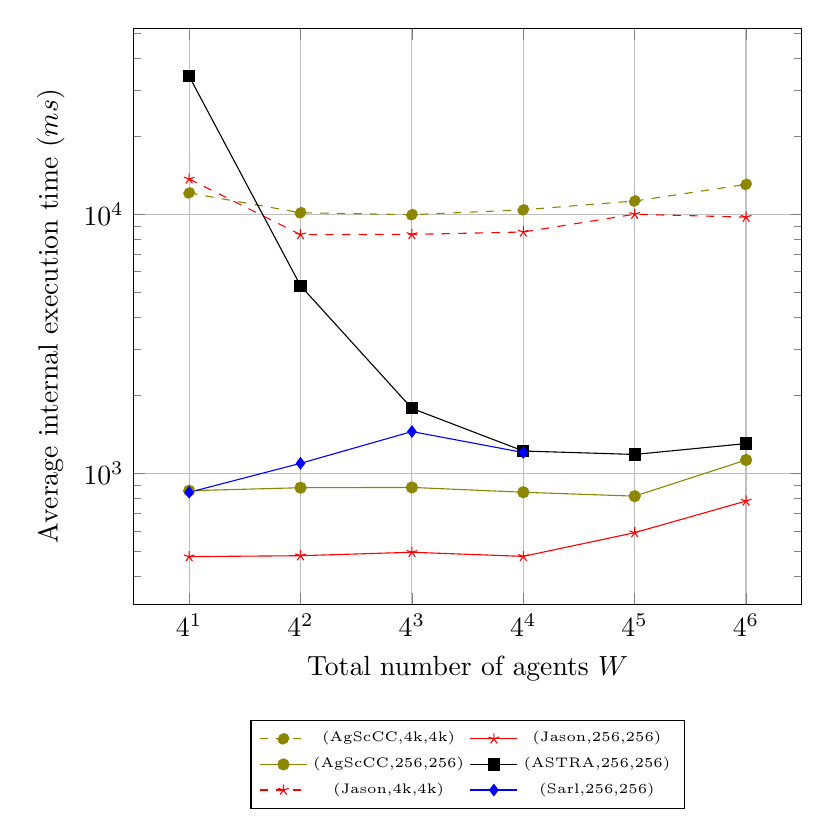
\begin{tikzpicture}
\begin{axis} [
scale only axis,
    width=0.70\textwidth,
    grid=major,
    transpose legend,
		legend columns=3,
		legend style={at={(0.5,-0.2)},anchor=north,font=\tiny},
    xmode=log,
    log basis x={4},
    ymode=log,
    log basis y={10},
    xlabel={Total number of agents $W$},
    ylabel={Average internal execution time ($ms$)},
    % cycle list name=
]
\addplot[mark=*,olive,dashed,error bars/.cd,y dir=both,y explicit
    ]
    coordinates {
(4 , 12064.0) %+- (654.172080657002 , 654.172080657002)
(16 , 10118.9) %+- (350.159471606232 , 350.159471606232)
(64 , 9943.9) %+- (233.08341377665155 , 233.08341377665155)
(256 , 10383.7) %+- (395.6162703091638 , 395.6162703091638)
(1024 , 11228.4) %+- (284.6249774313171 , 284.6249774313171)
(4096 , 13013.5) %+- (1324.0409736862375 , 1324.0409736862375)
    };
    \addlegendentry{(AgScCC,4k,4k)}
    
    \addplot[mark=*,olive,error bars/.cd,y dir=both,y explicit
    ]
    coordinates {
(4 , 857.1) %+- (98.22134866378761 , 98.22134866378761)
(16 , 880.3) %+- (70.18396461364155 , 70.18396461364155)
(64 , 882.6) %+- (119.83340287434235 , 119.83340287434235)
(256 , 845.5) %+- (105.0124331263261 , 105.0124331263261)
(1024 , 816.8) %+- (42.871383877308595 , 42.871383877308595)
(4096 , 1126.1) %+- (124.52170716608231 , 124.52170716608231)
    };
    \addlegendentry{(AgScCC,256,256)}
    
 
    \addplot[mark=star,red,dashed,error bars/.cd,y dir=both,y explicit
    ]
    coordinates {
   (4 , 13658.3) %+- (252.6855973559061 , 252.6855973559061)
(16 , 8329.5) %+- (164.36291146930523 , 164.36291146930523)
(64 , 8345.8) %+- (150.9273555942284 , 150.9273555942284)
(256 , 8527.7) %+- (150.2908661377811 , 150.2908661377811)
(1024 , 9984.2) %+- (209.81356803918408 , 209.81356803918408)
(4096 , 9729.8) %+- (1202.9822028678224 , 1202.9822028678224)
    };
    \addlegendentry{(Jason,4k,4k)}
    \addplot[mark=star,red,error bars/.cd,y dir=both,y explicit
    ]
    coordinates {
(4 , 477.4) %+- (13.133502536981096 , 13.133502536981096)
(16 , 481.3) %+- (14.14252845537569 , 14.14252845537569)
(64 , 496.3) %+- (22.90584593019384 , 22.90584593019384)
(256 , 478.5) %+- (23.665492928640965 , 23.665492928640965)
(1024 , 590.6) %+- (28.47298914956263 , 28.47298914956263)
(4096 , 782.5) %+- (30.938110263341336 , 30.938110263341336)
};
    \addlegendentry{(Jason,256,256)}
        \addplot[mark=square*,black,error bars/.cd,y dir=both,y explicit
    ]
    coordinates {
(4 , 34001.7) %+- (771.5794839159475 , 771.5794839159475)
(16 , 5293.5) %+- (330.20540745286274 , 330.20540745286274)
(64 , 1780.7) %+- (23.002656851377456 , 23.002656851377456)
(256 , 1219.4) %+- (27.597101297056543 , 27.597101297056543)
(1024 , 1182.8) %+- (18.972494710911253 , 18.972494710911253)
(4096 , 1302.7) %+- (29.95570804445197 , 29.95570804445197)

        };
    \addlegendentry{(ASTRA,256,256)}
    
       
    \addplot[mark=diamond*,blue,error bars/.cd,y dir=both,y explicit
    ]
    coordinates {
    (4 , 845.2222222222222) %+- (154.7447719454342 , 154.7447719454342)
    (16 , 1093.111111111111) %+- (619.9662177176359 , 619.9662177176359)
    (64 , 1449.5) %+- (790.6629075233853 , 790.6629075233853)
    (256 , 1203.2) %+- (1067.3895258995192 , 1067.3895258995192)
    };
    \addlegendentry{(Sarl,256,256)}
    

\end{axis}
\end{tikzpicture}
\caption{Token ring results for each (framework, $T, N$)}
\label{fig:token1}
\end{figure}%
\begin{figure}[tb!]
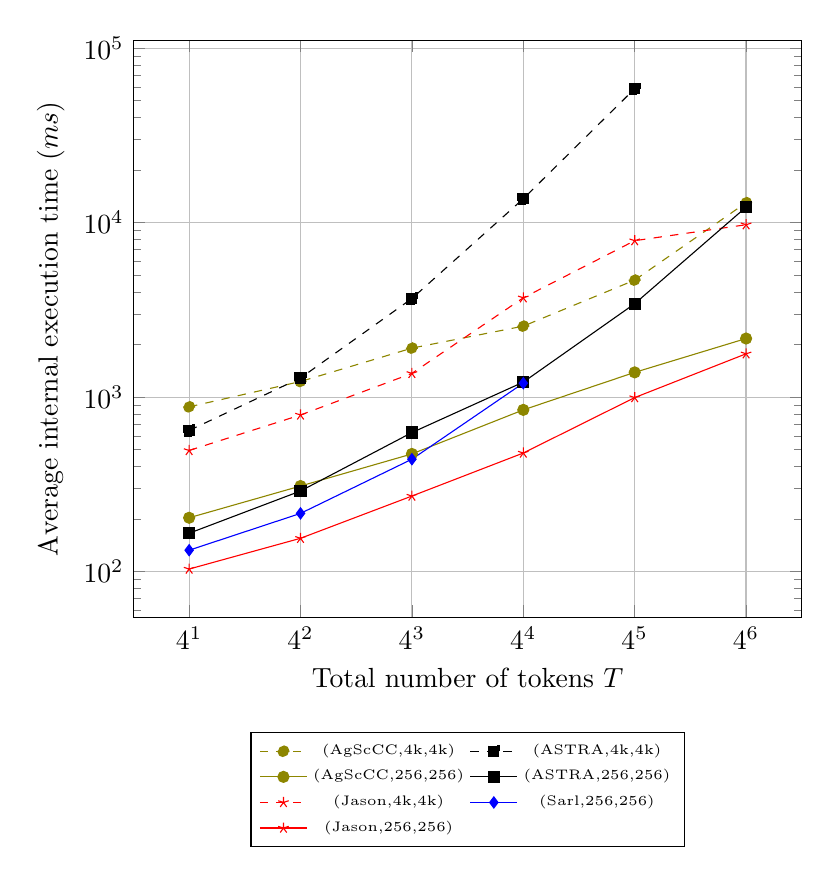
\begin{tikzpicture}
\begin{axis} [
scale only axis,
    width=0.7\textwidth,
    grid=major,
    transpose legend,
		legend columns=4,
		legend style={at={(0.5,-0.2)},anchor=north,font=\tiny},
    xmode=log,
    log basis x={4},
    ymode=log,
    log basis y={10},
    xlabel={Total number of tokens $T$},
    ylabel={Average internal execution time ($ms$)},
    cycle list name=black white
]

\addplot[mark=*,olive,dashed
    ]
    coordinates {
    (4 , 879.8)
(16 , 1229.2)
(64 , 1909.6)
(256 , 2552.4)
(1024 , 4684.5)
(4096 , 13013.5)
    };
    \addlegendentry{(AgScCC,4k,4k)}
    
    \addplot[mark=*,olive
    ]
    coordinates {
    (4 , 203.6)
    (16 , 309.5)
    (64 , 472.7)
    (256 , 845.5)
    (1024 , 1386.8)
    (4096 , 2167.5)
    };
    \addlegendentry{(AgScCC,256,256)}
    \addplot[mark=star,red,dashed
    ]
    coordinates {
    (4 , 494.8)
(16 , 790.4)
(64 , 1368.1)
(256 , 3710.7)
(1024 , 7884.8)
(4096 , 9729.8)
    };
    \addlegendentry{(Jason,4k,4k)}
    \addplot[mark=star,red
    ]
    coordinates {
    (4 , 103.5)
(16 , 155.3)
(64 , 271.2)
(256 , 478.5)
(1024 , 994.2)
(4096 , 1772.2)
};
    \addlegendentry{(Jason,256,256)}
    
    \addplot[mark=square*,black,dashed
    ]
    coordinates {
    (4 , 644.4)
(16 , 1287.1)
(64 , 3674.8)
(256 , 13711.6)
(1024 , 58593.0)
        };
    \addlegendentry{(ASTRA,4k,4k)}
    
        \addplot[mark=square*,black
    ]
    coordinates {
    (4 , 166.0)
(16 , 289.8)
(64 , 626.6)
(256 , 1219.4)
(1024 , 3432.0)
(4096 , 12273.7)
        };
    \addlegendentry{(ASTRA,256,256)}
    
       
    \addplot[mark=diamond*,blue
    ]
    coordinates {
    (4 , 132.7)
    (16 , 215.7)
    (64 , 440.9)
    (256 , 1203.2)
    };
    \addlegendentry{(Sarl,256,256)}

\end{axis}
\end{tikzpicture}
\caption{Token ring results for each (framework,$W,N$)}

\label{fig:token2}
\end{figure}


\begin{figure}
    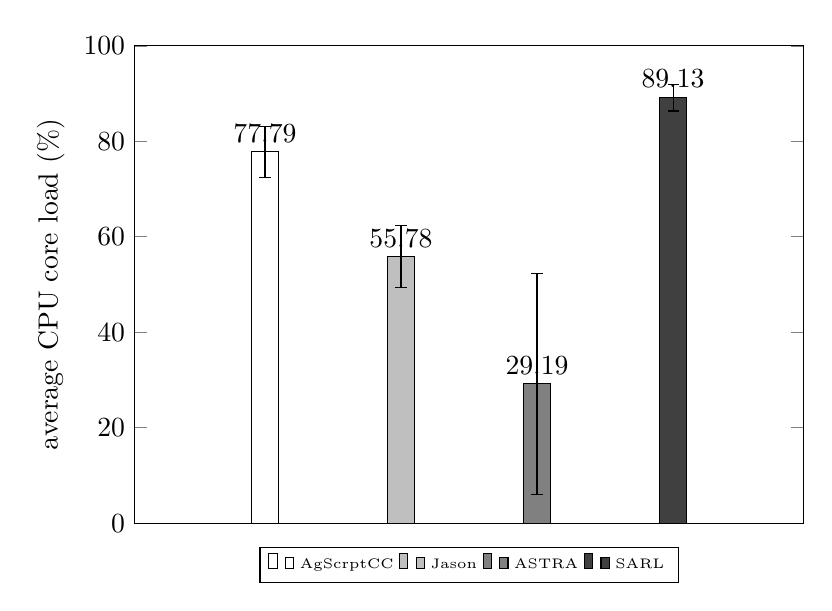
\begin{tikzpicture}
\begin{axis}[
    scale only axis,
    height=0.5\textwidth,
    width=0.7\textwidth,
    ybar,
    enlarge x limits=0.15,
    legend style={at={(0.5,-0.05),font=\tiny},
      anchor=north,legend columns=-1},
    ylabel={average CPU core load (\%)},
    xmin=-1, xmax=4,
    xtick style={draw=none},
     xticklabels={,},
    nodes near coords,
    nodes near coords align={vertical},
    ymin=0,
    ymax=100
    ]
\addplot[fill=black!0, error bars/.cd, y dir=both, y explicit] coordinates {(0,77.78875) +- (5.312416741175037,5.312416741175037)};
\addplot[fill=black!25,error bars/.cd,y dir=both,y explicit] coordinates {(1,55.78125) +-(6.486383053627206,6.486383053627206)};
\addplot[fill=black!50,error bars/.cd,y dir=both,y explicit] coordinates {(2,29.18625) +-(23.211414457534154,23.211414457534154)};
\addplot[fill=black!75,error bars/.cd,y dir=both,y explicit] coordinates {(3,89.13125) +-(2.790913631127873,2.790913631127873)};
\legend{AgScrptCC,Jason,ASTRA,SARL}
\end{axis}
\end{tikzpicture}
     \caption{CPU load (average and standard deviation on 8 cores) in token ring with $N=4k$, $T=256$ and $W=256$}
    \label{fig:cpu_load_token1}
     
        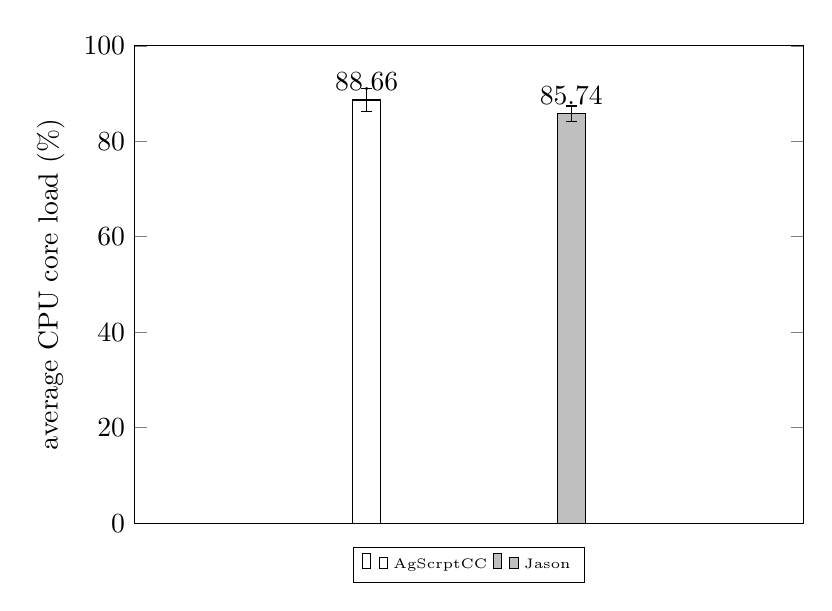
\begin{tikzpicture}
\begin{axis}[
    scale only axis,
    width=0.7\textwidth,
    height=0.5\textwidth,
    ybar,
    enlarge x limits=0.15,
    legend style={at={(0.5,-0.05),font=\tiny},
      anchor=north,legend columns=-1},
    ylabel={average CPU core load (\%)},
    xmin=-1, xmax=2,
    xtick style={draw=none},
    xticklabels={,,,},
    nodes near coords,
    nodes near coords align={vertical},
    ymin=0,
    ymax=100
    ]
\addplot[fill=black!0, error bars/.cd, y dir=both, y explicit] coordinates {(0,88.6575) +-(2.4864003978712743,2.4864003978712743)};
\addplot[fill=black!25,error bars/.cd,y dir=both,y explicit] coordinates {(1,85.73875000000001) +-(1.6477440981797706,1.6477440981797706)};

\legend{AgScrptCC,Jason}
\end{axis}
\end{tikzpicture}
     \caption{CPU load (average and standard deviation on 8 cores) in token ring with $N=4k$, $T=4k$ and $W=4k$}
    \label{fig:cpu_load_token2}
    
\end{figure}

\begin{figure}[tb!]
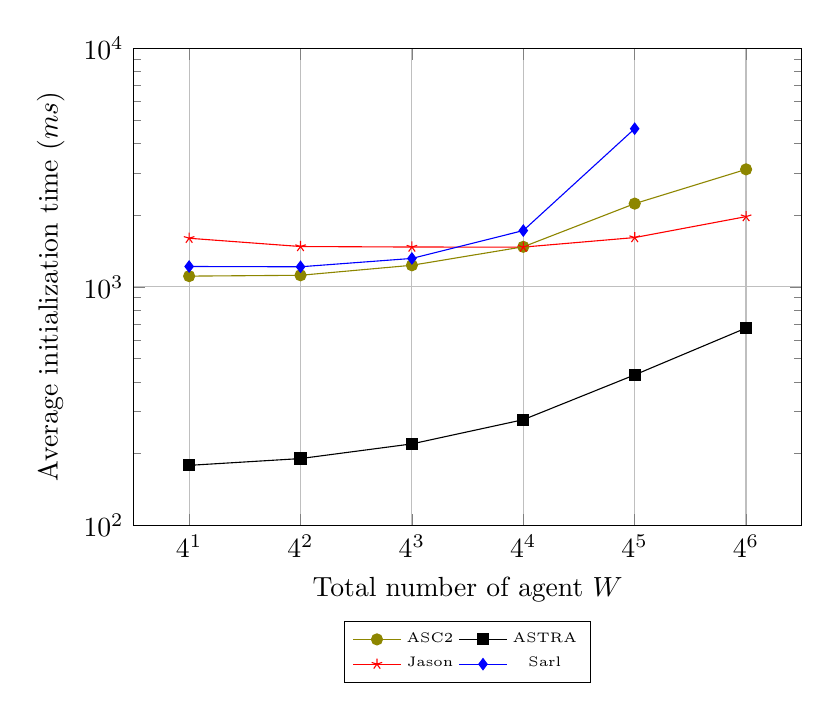
\begin{tikzpicture}
\begin{axis} [
    scale only axis,
    width=0.7\textwidth,
    height=0.5\textwidth,
    grid=major,
    transpose legend,
		legend columns=2,
		legend style={at={(0.5,-0.2)},anchor=north,font=\tiny},
    xmode=log,
    log basis x={4},
    ymode=log,
    log basis y={10},
    ymin=100,
    ymax=10000,
    xlabel={Total number of agent $W$},
    ylabel={Average initialization time ($ms$)},
    cycle list name=black white
]


    \addplot[mark=*,olive
    ]
    coordinates {
    (4 , 1108.8999999999999)
    (16 , 1118.0)
    (64 , 1231.2)
    (256 , 1471.6)
    (1024 , 2231.5)
    (4096 , 3106.0)
    };
    \addlegendentry{ASC2}
    
    \addplot[mark=star,red
    ]
    coordinates {
    (4 , 1597.7)
    (16 , 1475.5)
    (64 , 1468.2)
    (256 , 1467.1999999999998)
    (1024 , 1608.7)
    (4096 , 1969.0)
};
    \addlegendentry{Jason}
    

    
        \addplot[mark=square*,black
    ]
    coordinates {
(4 , 178.7)
(16 , 190.8)
(64 , 219.79999999999998)
(256 , 277.6)
(1024 , 427.70000000000005)
(4096 , 672.0999999999999)
        };
    \addlegendentry{ASTRA}
    
       
    \addplot[mark=diamond*,blue
    ]
    coordinates {
    (4 , 1216.7)
    (16 , 1213.6000000000001)
    (64 , 1315.3999999999999)
    (256 , 1721.2)
    (1024 , 4599.25)
    };
    \addlegendentry{Sarl}

\end{axis}
\end{tikzpicture}
\caption{Initialization time in token ring with $T=4$, $N=4$}

\label{fig:init1}
\end{figure}

\subsection{Chameneos Redux}
The second benchmark is adopted from \cite{Kaiser2003} and is a test intended to capture the effects of one limiting point to the execution framework. The scenario consists of $C$ chameneo creatures living in the jungle; they can go to a common place to meet other creatures and \textit{mutate} with them. Each creature has a color assigned to it from a color pool and after mutation its colour changes based on the color of the other creature it met. These meetings should happen for a total number of $N$ times. To run this benchmark a program should:
\begin{itemize}
    \item create $C$ differently colored (blue, red, yellow), differently named, concurrent chameneo creatures
    \item write all the possible complementary color combinations;
    \item write the initial color of each creature;
    \item each creature will repeatedly go to the meeting place and meet, or wait to meet, another chameneo;
    \item both creatures will change color to complement the color of the chameneo that they met;
    \item after $N$ meetings have taken place, for each creature write the number of creatures met and the number of times the creature met a creature with the same name (should be zero).
    \item the program finishes when $N$ meetings have happened.
\end{itemize}


The experiment was performed with the set of variables $C=\{64,256,1k,4k\}$ and $N=\{1k,4k,16k,64k\}$. This provide us with $20$ different configurations for each framework. All tests were given a $1$ minute time limit and it is considered a timeout after that.


\subsubsection{Implementation Notes} In all implementations a \textit{broker} agent is present that acts as the meeting point for chameneos. This agent is the main point of this benchmark as it will be constantly under high number of requests from the chameneos agents.

\subsubsection{Results} 

The first view on the results is presented in Figure \ref{fig:cham1}. In this setting the number of meetings $N$ is kept constant at two values $4k$ and $64k$ whilst the number of chameneos is the variable. The results show that Jason and ASC2 scale well with the number of agents while ASC2 performs marginally better in the $N=64k$ test. Sarl and ASTRA suffer from the higher number of agents to the point that Sarl could finish both tests only up to $C=1k$ agents while ASTRA finishing $N=64k$ test only in the $C=64$ agents setting.

Figure \ref{fig:cham2} presents another view on the results. This time the number of chameneos $C$ is kept constant at $256$ and $4k$, whilst the number of meetings $N$ is the variable. Sarl could only finish the $C=256$ test while ASTRA could only finish it up to $N=16k$ and timing out after that. ASTRA was also only able to finish the $C=4k$ test with $C=64$ number chameneos. ASC2 and Jason both completed the tests with linear scaling, with ASC2 outperforming Jason slightly in the $C=4k$ test. This shows that both Jason and ASC2 can handle higher levels of concurrency in the broker agent w.r.t. the increasing number of concurrent requests.

\begin{figure}[tb!]
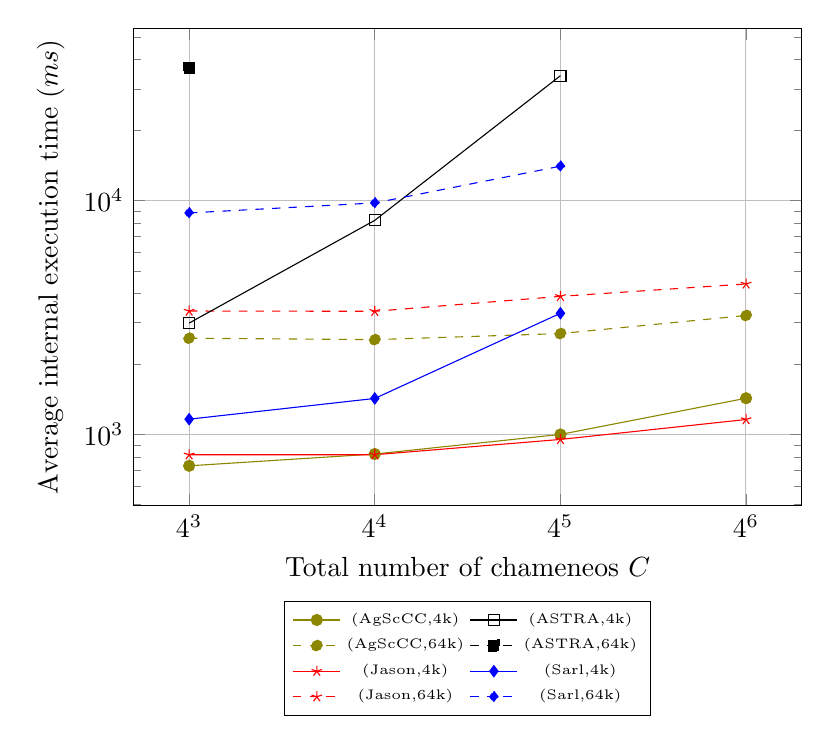
\begin{tikzpicture}
\begin{axis} [
    scale only axis,
    width=0.7\textwidth,
    height=0.5\textwidth,
    grid=major,
    transpose legend,
		legend columns=4,
		legend style={at={(0.5,-0.2)},anchor=north,font=\tiny},
    xmode=log,
    log basis x={4},
    ymode=log,
    log basis y={10},
    xlabel={Total number of chameneos $C$},
    ylabel={Average internal execution time ($ms$)},
    cycle list name=black white
]


    \addplot[mark=*,olive
    ]
    coordinates {
(64 , 733.5)
(256 , 823.8)
(1024 , 999.0)
(4096 , 1426.8)
    };
    \addlegendentry{(AgScCC,4k)}
    
\addplot[mark=*,olive,dashed
    ]
    coordinates {
    (64 , 2576.7)
(256 , 2540.6)
(1024 , 2697.0)
(4096 , 3222.8)
    };
    \addlegendentry{(AgScCC,64k)}
        \addplot[mark=star,red
    ]
 coordinates {
 (64 , 817.5)
(256 , 818.2)
(1024 , 950.9)
(4096 , 1157.2)
};
    \addlegendentry{(Jason,4k)}
    \addplot[mark=star,red,dashed
    ]
    coordinates {
(64 , 3367.3)
(256 , 3358.6)
(1024 , 3891.0)
(4096 , 4396.3)
    };
    \addlegendentry{(Jason,64k)}

        \addplot[mark=square,black
    ]
    coordinates {
(64 , 2990.9)
(256 , 8224.0)
(1024 , 34161.1)
        };
    \addlegendentry{(ASTRA,4k)}
    
    \addplot[
    mark=square*,black,dashed
    ]
    coordinates {
    (64 , 36860.8)
        };
    \addlegendentry{(ASTRA,64k)}   
    
    \addplot[mark=diamond*,blue
    ]
    coordinates {
        (64 , 1160.8)
    (256 , 1423.9)
    (1024 , 3293.9)
    };
    \addlegendentry{(Sarl,4k)}
    
    \addplot[mark=diamond*,blue,dashed]
    coordinates {
        (64 , 8846.6)
        (256 , 9760.6)
        (1024 , 14014.9)
    };
    \addlegendentry{(Sarl,64k)}
    


\end{axis}
\end{tikzpicture}
\caption{Chameneos redux results for each (framework, $N$)}

\label{fig:cham1}
\end{figure}

\begin{figure}[tb!]
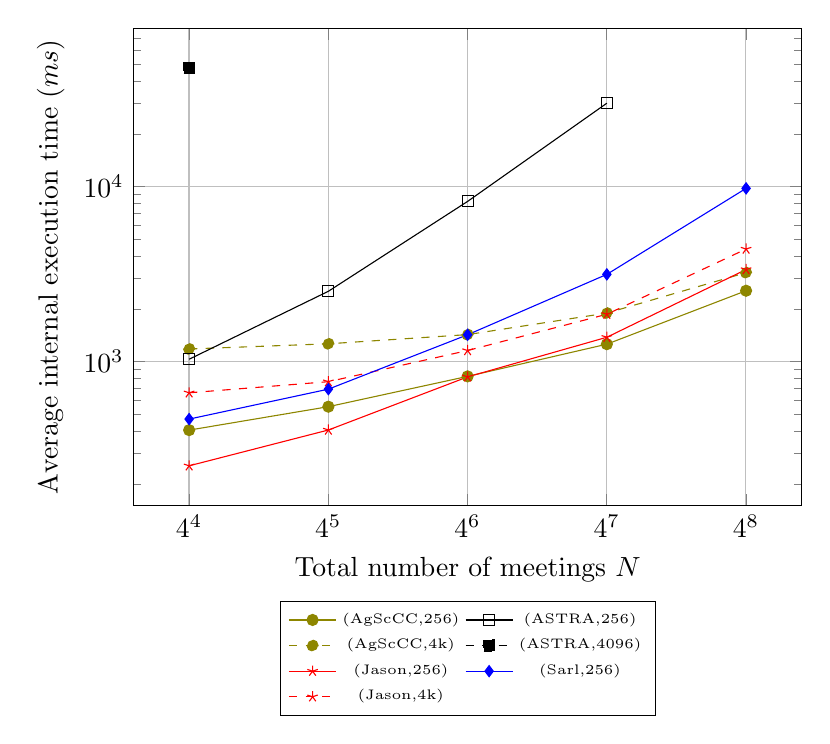
\begin{tikzpicture}
\begin{axis} [
scale only axis,
    width=0.7\textwidth,
    height=0.5\textwidth,
    grid=major,
    transpose legend,
		legend columns=4,
		legend style={at={(0.5,-0.2)},anchor=north,font=\tiny},
    xmode=log,
    log basis x={4},
    ymode=log,
    log basis y={10},
    xlabel={Total number of meetings $N$},
    ylabel={Average internal execution time ($ms$)},
    cycle list name=black white
]

\addplot[mark=*,olive
    ]
    coordinates {
(256 , 406.3)
(1024 , 552.9)
(4096 , 823.8)
(16384 , 1258.0)
(65536 , 2540.6)
    };
    \addlegendentry{(AgScCC,256)}
    
    \addplot[mark=*,olive,dashed
    ]
    coordinates {
(256 , 1180.9)
(1024 , 1264.3)
(4096 , 1426.8)
(16384 , 1893.3)
(65536 , 3222.8)
    };
    \addlegendentry{(AgScCC,4k)}
    \addplot[mark=star,red
    ]
    coordinates {
(256 , 254.1)
(1024 , 406.9)
(4096 , 818.2)
(16384 , 1377.9)
(65536 , 3358.6)
    };
    \addlegendentry{(Jason,256)}
    \addplot[mark=star,red,dashed
    ]
 coordinates {
(256 , 663.7)
(1024 , 768.3)
(4096 , 1157.2)
(16384 , 1864.9)
(65536 , 4396.3)
};
    \addlegendentry{(Jason,4k)}
    
    \addplot[mark=square,black
    ]
    coordinates {
(256 , 1031.8)
(1024 , 2522.3)
(4096 , 8224.0)
(16384 , 29916.6)
        };
    \addlegendentry{(ASTRA,256)}
    
        \addplot[mark=square*,black,dashed
    ]
    coordinates {
(256 , 47535.6)
        };
    \addlegendentry{(ASTRA,4096)}
    
       
    \addplot[mark=diamond*,blue
    ]
    coordinates {
    (256 , 469.7)
(1024 , 696.3)
(4096 , 1423.9)
(16384 , 3150.7)
(65536 , 9760.6)
    };
    \addlegendentry{(Sarl,256)}

   \addplot[mark=diamond*,blue]
    coordinates {

    };
    \addlegendentry{(Sarl,4096)}

\end{axis}
\end{tikzpicture}
\caption{Chameneos redux results for each (framework,$C$)}

\label{fig:cham2}
\end{figure}



\subsection{Service Point}
This last benchmark is not about performance. Rather, it is designed to illustrate the differences between the execution in a \textit{step-based} framework like Jason in contrast to a compilation-based framework like ASC2, focusing on how they handle actions (namely time-consuming primitive actions) specified outside their DSL. The scenario of this benchmark consists of one service point and $N$ number of consumers. Each consumer sends $R$ requests to the service point and waits for the response. The service point needs a random  amount of time $t$ ($0 \le t \le 5000$ ms) to process each request. A simple \verb+Thread.sleep(t)+ is used to mimic thread time consumption. To run this benchmark a program should
\begin{itemize}
    \item create $1$ service point and $N$ service consumers.
    \item each consumer will send $R$ number of requests to the service point
    \item the program finishes when all of the $R*N$ requests have been responded 
\end{itemize}
The experiment was done only on Jason and ASC2 with variables $N=\{1,4,16\}$ and $R=\{1,4,16\}$. With respect to total number of request $R*N$, this gives us with 5 unique configurations. To account for the non-determinism added by the randomization each configuration is executed for $100$ times.

\subsubsection{Results}
The results of this experiment are presented in Figure \ref{fig:ping_pong1}. Jason performs much worse in this scenario, as it is not being able to finish the $256$ requests within a $200$ seconds timeout. This is even more strange as in our setting Jason is set to use $8$ threads and ASC2 to $6$ and by looking at the results we can see that ASC2 is always using the thread times completely but Jason is not. The reason for this is that Jason uses a \textit{sequential} reasoning cycle inside each agent; %in a symbolic way; 
at every reasoning cycle, a Jason agent takes the next step from each of its intentions and executes them. The reasoning cycle ends when all intentions execute one step. This means that if in the reasoning cycle of an agent one of these steps is a time-consuming primitive action, the whole cycle will be blocked\footnote{Jason provides extra built-in directives like \texttt{.wait} to mimic unblocking suspension of intentions but that is beyond the context of this benchmark.}. On the contrary a compiled agent does not have any notion of steps at run-time and the parallelism between intentions of the agent is also handled by the underlying concurrency model, in this case the Actor model. This matter is further discussed in \ref{subsec:par}.

\begin{figure}[bt!]
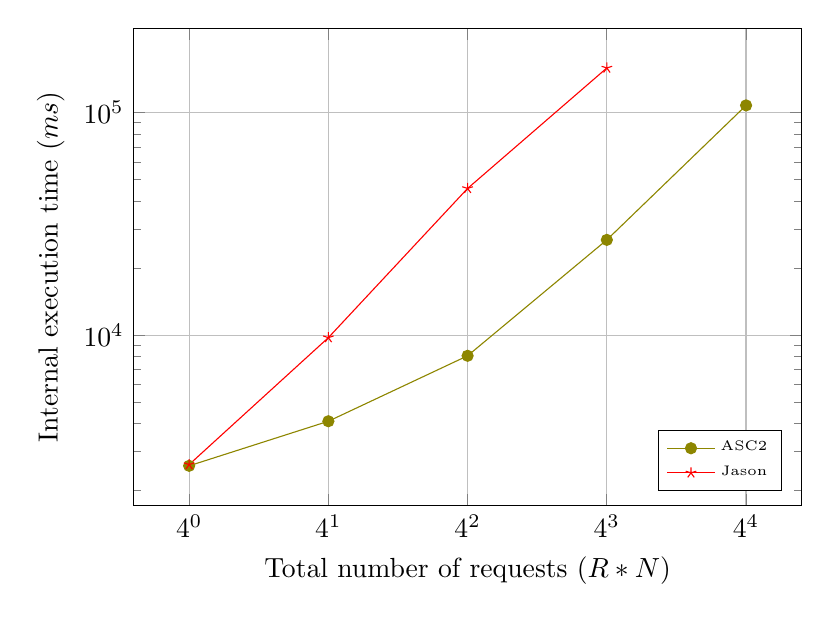
\begin{tikzpicture}
\begin{axis} [
    scale only axis,
    width=0.7\textwidth,
    height=0.5\textwidth,
    grid=major,
    legend pos=south east,
    legend style = {font=\tiny},
    xmode=log,
    log basis x={4},
    ymode=log,
    log basis y={10},
    xlabel={Total number of requests ($R*N$)},
    ylabel={Internal execution time ($ms$)},
    cycle list name=black white
]
\addplot[mark=*,olive
    ]
    coordinates {
    (1,2586.46)(4,4101.450000000001)(16,8072.993333333333)(64,26780.0)(256,107672.52)
    };
    \addlegendentry{ASC2}
    \addplot[mark=star,red
    ]
    coordinates {
    (1,2619.74)(4,9738.456756756757)(16,45602)(64,158538)
    };
    \addlegendentry{Jason}
\end{axis}
\end{tikzpicture}
\caption{Service point scenario results}
\label{fig:ping_pong1}
\end{figure}

\section{Discussion}
\label{sec:discussion}
This chapter presents and evaluates a framework for an AOP language based on AgentSpeack(L) relying on compilation. Compilation in this context is not novel as it has been used previously by other AOP frameworks like SARL \cite{Sarl} and ASTRA \cite{Astra}. The novelty of this work lies in two aspects. First, unlike SARL and ASTRA, that use a DSL very close to their underlying language (Java), ASC2 uses a logic-based DSL close to AgentSpeak(L). %\Gio{but in principle,} 
As our pipeline starts from an \textit{antlr} grammar, in principle 
the current DSL can be replaced by any other AOP language that can be mapped to the ASC2 abstract execution architecture. Second, our approach maps the DSL into an architecture that exploits the Actor model. This means that not only the final executable model is more robust, because it takes advantage of the established concurrency model and the maturity of the libraries implementing the Actor model (e.g, Akka), but also that the translation itself is an open process, so its product becomes in principle more understandable for the programmer.


\subsection{Performance}
The execution model of ASC2 is closer to Sarl and ASTRA than to Jason (see \ref{subsec:par}), but, as shown by the benchmarks, it is substantially outperforming both Sarl and ASTRA. At the same time, ASC2 performance was below what we expected before running these experiments. Investigating possible causes by profiling the execution of benchmarks, we found out that a considerable amount of execution time is spent on the blocking due to \textit{synchronized query calls} to the belief base. These calls had to be synchronized because Prolog engines like \textit{Styla} and \textit{tuProlog} \cite{tuprolog} (another candidate solution we tested for handling belief bases) are inherently made for single thread access. Even a simple \textit{read} query to a Prolog engine still counts as \textit{write} access because of the backtracking.
%Interestingly enough Jason does not have any issue with this because, as presented in \ref{subsec:par}, the intentions of one Jason agent are only symbolically concurrent, therefore there will be no need to synchronize belief base access as they are ultimately sequential. 
We believe once this issue is addressed the performances of ASC2 will greatly improve.


\subsection{Language}

Although all of the considered frameworks propose DSLs to program reactive agents, their bases are different. %the ideas behind them differ.
Agent-ScriptCC's DSL is based on AgentSpeak(L), which gives to the language a logic-oriented flavour; this is also the case for Jason, and both frameworks can take advantage of Prolog-style terms and expressions. ASTRA's DSL is also based on concepts defined in AgentSpeak(L) but with more syntactic resemblance to Java. Sarl's language does not try to be a logic-based language, therefore it does not contain components corresponding to terms or expressions; it is rather very close to Java.

% Noone asked!
%\subsubsection{Type system}
%The desirability of a language to be typed depends on the application it is used for. Among these frameworks Jason and ASC2 are un-typed while ASTRA and Sarl are typed.% Note that Sarl allows for shared declaration of event types but in ASTRA programs, every formula needs to be introduced as a type in each agent program.

\subsection{Execution and Parallelism}
\label{subsec:par}
As a common ground, all these frameworks are used to specify reactive agents, but they differ in how the agent's (re)actions are executed. The most particular solution comes with Jason which uses the concept of \textit{steps}. The Jason interpreter treats each symbolic step/instruction in a plan of a reactive rule as a single unit of execution, and emulates an imperative program by executing them in a sequence in consecutive reasoning cycles. In contrast, in the other three frameworks, the steps of the reactive rules are already imperative programs ready to be executed. The approach taken by Jason has important consequences especially when agents execute multiple parallel threads of work (intentions) at the same time. This concept is examined more in detail in section \ref{sec_bench} and in \cite{Astra}.

\subsection{Access to the Lower-Level Language}
One of the motivations behind developing ASC2 has been to enable access to libraries defined in the underlying general-purpose programming language of choice in a easy and seamless way. In our view this impacts the usability of the framework in larger applications. Leading by an example, consider a programmer that needs to call the Java function \verb+Thread.sleep(1)+ in a reactive rule. In Jason one needs to create an extra class extending one of Jason's internal classes (\verb+Agent+, \verb+Action+ or \verb+Environment+) and define a method that wraps this low level function and then call the wrapping method from the agent program. In ASTRA it is almost the same as Jason and one needs to create a class extending the type \verb+Module+, wrap this function inside a method, and annotate it appropriately to be able to call it from the agent program. On the opposite side, this is entirely different for Sarl and ASC2, as one can simply call this function directly from the agent program. In case of ASC2 this can be done with \verb+#Thread.sleep(1)+.

\subsection{Communication}
The communication in ASC2 is entirely externalized, both for agent-to-agent and agent-to-environment communication. In the current implementation communication between agents uses Akka's internal message system but this can easily be replaced with any other type of communication mechanism, e.g. by using a message queue (\textit{MQ}) to be able to execute the agents in a distributed setting. For the other frameworks, externalization is possible, but requires specific wrappers to the communication infrastructures (Jason with JADE).

\section{Conclusion and Future developments}
%The slowly but steadily increasing interest in languages based on BDI or functionally similar architectures for virtual assistants, robotics, (serious) gaming, as well as for social simulations, hints that there is a general consensus that these solutions might be suitable to reproduce human-like reasoning, or rather human-intelligible computation. So far, the majority of contributions in this area were concerned mostly by the logical aspects of the problem rather than its computational aspects \cite{Herzig2017}. Indeed, intentional (or alternatively \textit{policy-based}, or also \textit{purpose-driven}) programming (dealing with why) aims to provide a different level of abstraction w.r.t. declarative programming (dealing with what, or the outcome) and imperative programming (dealing with how, or operations), and understanding its specificities and identifying sound logical properties are crucial passages. 

The slowly but steadily increasing interest in programming languages based on BDI or functionally similar architectures for virtual assistants, robotics, (serious) gaming, as well as for social simulations, hints that there is a general consensus that these solutions might be suitable to reproduce human-like reasoning, or rather human-intelligible computation. 

Historically, the majority of contributions in this area were concerned mostly by the logical aspects of the problem rather than its computational aspects \cite{Herzig2017}. However, more recent contributions %made clear the presence of relevant 
revealed the presence of issues w.r.t. computational performance and compatibility to modern environments and tools, motivating efforts to redevelop existing BDI frameworks according to best practices \cite{LJ,pyson}. Looking at intentional programming in the longer term, we need to acknowledge that operational settings differ from the typical low-scale simulation setting in which it is used today. Besides a difference in scale, components can also be fully distributed. %, and time synchronization cannot be guaranteed (or at least only to a certain extent). 
Because of this, a future target feature of ASC2 will be the capability to deploy and execute agents in distributed settings. This seems to be an achievable objective as there are already approaches available to run actors in distributed environments.% Another related concept to be investigated, both at theoretical and practical levels, is to extend event-based reactivity of the agents into stream-based reactivity, to enable agent programs to be used for modern data-centric applications.

An initial, additional motivation of using an actor-oriented architecture for the intentional agents is that by having this extra level of abstraction the agent become more modular, enabling the augmentation of agents with complementary machinery like using AI modules \cite{Singh2011IntegratingLI}, normative reasoning modules \cite{meneguzzi2009norm}, planning (e.g. HTN, STRIPS) modules \cite{meneguzzi_de_silva_2015} and preference checking modules \cite{Visser2016,Mohajeri2019}. Defining  adequate interfaces to support the different types of add-ons for ASC2 agents will be investigated in the future.

The present work acts as a starting block towards this path. The benchmarks reported here demonstrates that, despite the initial maturity level of the framework, ASC2 is already competitive against existing frameworks, motivating further exploration.

%Furthermore, agents might encapsulate other AI modules (e.g. machine learning-based) that are better executed if concurrency is safe. % This abstraction level is relevant also because purpose is one of the elements that enable to recognise e.g. legitimate processing (e.g. according to GDPR). Most applications in this area introduce purpose only as meta-data of requests, and in doing so they break the connection between performance and (intended) outcome. In principle, recovering this link would facilitate the maintenance of applications as well as the social functioning of the infrastructure.

%Furthermore, we believe there are still mechanisms to be explored at intentional level of agents, e.g, addressing the gap between goals and desires \cite{Dignum2002} or having explicit preferences as part of the script \cite{Mohajeri2019}.
 %(e.g. agent's desires are for the most considered only in the reduced form of goals)
 %we decided to follow a different path than building from scratch yet another framework. We decided instead to experiment with the reuse of established, robust components as actors. 
% By approaching an intentional agent as a system of actors, %designers are enabled
 %we can test different theories in a more structured way by mapping them to externally programmable strategies for the actor-based architecture, %: even if these actors are functionally constrained by 
 %either by recomposing the abstract architecture or by restructuring the interactions between (agent-internal) actors.
 
 %Second, by establishing a direct mapping of the scripts to the underlying language, programmers can enjoy of a direct connection with existing ecologies of tools such as debuggers, profilers, build tools, etc. an option that in principle facilitates adoption. The partial success of ASC2---still at its infancy---on the various benchmarks investigated here confirms us that this might be a viable path.
